\chapter{Experimental Setup, Models and Validation}
\label{chap5}
\textit{In this section we look at how we will set up our proposed solution, so that it can be replicated, as well as how we propose to validate the framework developed. We will look in detail at each of the three visualization themes (science, operations and community) in isolation.}
\vspace{2ex}\vfill
\minitoc
\newpage

\section{Scientific Portal}
The Scientific Portal is the cornerstone of the Data Everywhere project and is based on work already done in previous research and is primarily intended to convey trends and anomalies which would otherwise be obscured by traditional visualization techniques such as case pyramids and time series plots [cite 8]. The authors of that research propose the use of multi-panel (MP) graph to achieve this. The MP graph consists of an outcome pyramid, a time-series plot and an image plot (heat map) positioned on a single canvas where at least two or more graphs share at least one common axis. This design allows for the simultaneous visualization of population structure and temporal trend.

\subsection{Outcome Pyramid}

An outcome pyramid is similar to a population pyramid, a type of graph used to describe the age and sex composition of a population. An outcome pyramid describes the age and sex distribution of a population who have a particular health or disease outcome. The pyramid itself is basically two vertically juxtaposed histograms, one for males and another for females and a vertical axis common to the two histograms which displays age. This can be represented as single years or 5 year categories. The horizontal axis can display absolute counts or rates. The longer a bar extends from the vertical axis the greater the proportion or number of individuals in that age category.

When looking at outcome pyramids, three things should are deserving of attention: the overall shape of the pyramid, such as uniform, triangular or even inverted triangle; the presence or absence of symmetry by gender; and irregularities such as bumps or spikes in the cases [cite 8]. In of themselves, outcome pyramids provide a useful tool for assessing age and gender disparities in diseases. However, as noted in [cite 8], static outcome pyramids fail to display temporal changes, which can be quite extensive especially for infectious diseases with well pronounced seasonality.

\subsection{Time Series}

Time-series plots are used to visualise temporal trends and seasonal patterns in disease rates. For the time series to be informative, it must span a sufficiently long time frame and a carefully chosen unit of time (such as day, week, month or year). For many outbreak surveillance systems, a weekly time series is standard [insert citation]. However, INDEPTH sites were not structured for outbreak surveillance, rather they excel at trend surveillance, and therefore it makes more sense to choose a year as a unit of surveillance time in our case. The vertical axis in the time series can show either disease counts or rates. 

Although a well-constructed time series plot can show the temporal fluctuations in disease occurrence, interpretation of the fluctuations requires an assumption of equally distributed risk through the represented ages in the population. In reality diseases seldom affect all ages uniformly. This erroneous assumption can be partially alleviated by compiling time series plots for specific age groups, choosing a medium sized interval (5 year) [cite 8]. The added interactivity afforded by our web application allowed us to choose this option allowing a user to choose an age group of interest to visualise on the time series, thus adding a demographic dimension to it, whereas [cite 8] had a disaggregated time-series with no demographic dimension.

\subsection{Image Plot (Heat Map}

An image plot or heat map is a data visualization tool which can be used to graphically represent your data for at least three variables. At a basic level, they can be thought of as spreadsheets which have colours instead of numbers, whereby the colour of each cell or rectangle is related to the magnitude (count or rate) of the cell amount [cite 14]. In our case the first two variables age (age groups) and time (year) are represented by the vertical axis and horizontal axis respectively. The third variable is outcome count/rate (outcome being the disease or health outcome of interest) and it is represented by the different hues or saturation of colours within the plot.

New information previously obscured by outcome pyramids and time series plots can surface on using image plots, although reading the graph properly requires some training and practice [cite 8]

\begin{figure}[!ht] 
\centering
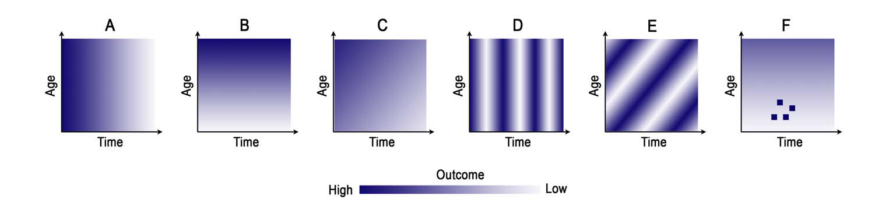
\includegraphics[scale=0.4]{./Chapter5/images/imageplots}
\caption{Typical patterns observed in image plots used to study the association between age, time and the disease/outcome of interest [cite 8]}
\label{fig1}
\end{figure}

Some typical patterns are shown in \ref{fig1}. Panel A shows a decrease in colour from left to right indicating a decrease in the outcome of interest over time, which is more or less uniform among all ages. 

Panel B shows a decrease in saturation from top to bottom showing an increase in relative risk of the outcome in older age groups irrespective of time. Another variation of B is its’ inverse, whereby the saturation is darker in the lower age groups and lighter in the older age groups, signifying increased relative risk in the younger age groups for that particular outcome. 

Panel C is a combination of both Panel A and Panel B in that the older age groups constantly remain at highest risk of the outcome of interest but this risk is gradually reducing over all age groups over time.

Panel D shows a striated pattern which is evidence of seasonality. The outcome of interest increases and wanes more or less evenly over all age groups periodically.

Panel E is a striated pattern which suggest a phenomenon known as the “age-cohort effect“. This is where there is an observable variation in the risk of a health outcome according to the year of birth [cite 15]. It is seen when an outcome is measured in the same cohort repeatedly and the outcome remains higher or lower in a particular group of subjects as they aged.

Lastly, panel F overall shows a similar pattern to pattern B whereby the outcome is increasingly higher as you go up the age groups, but relatively unchanging over time. However the four distinct clusters in the younger age group seen at specific periods in time within the panel could indicate an outbreak, due to the disproportionally high values of the outcome of interest.

The combination of these three types of plots, outcome pyramid, time series and heat map strategically juxtaposed onto a single canvas give us an MP graph (\ref{fig2} and \ref{fig3}).

\begin{figure}[!ht] 
\centering
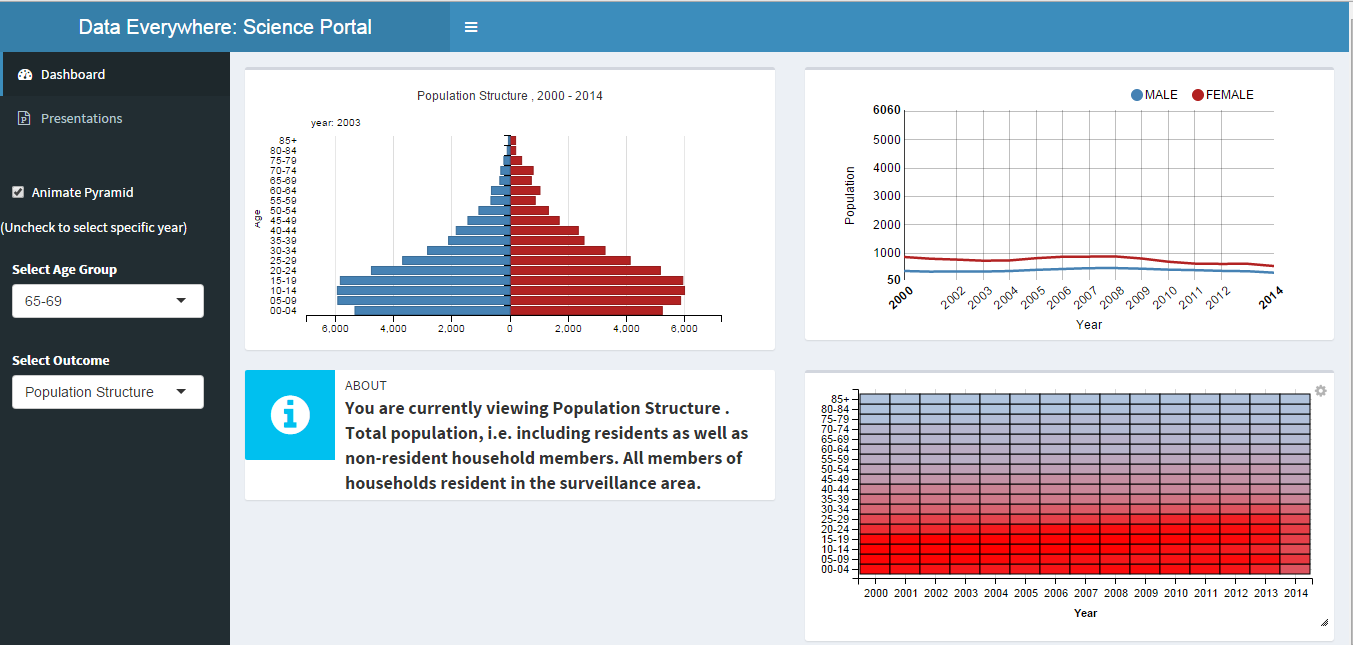
\includegraphics[scale=0.3]{./Chapter5/images/shinymp1}
\caption{MP graph showing the population structure of a population in a particular health and demographic surveillance site}
\label{fig2}
\end{figure}

In \ref{fig2}, the top left panel is an outcome pyramid which is set to dynamically change over time to animate the changes in the age and sex distribution. The top right panel is a time series showing the trend in the population disaggregated by sex for a particular age group (here the age group is 65-69, selected from a drop down menu on the left sidebar). The lower right panel shows a heat map which indicates a higher population density in the lower age groups. 

\begin{figure}[!ht] 
\centering
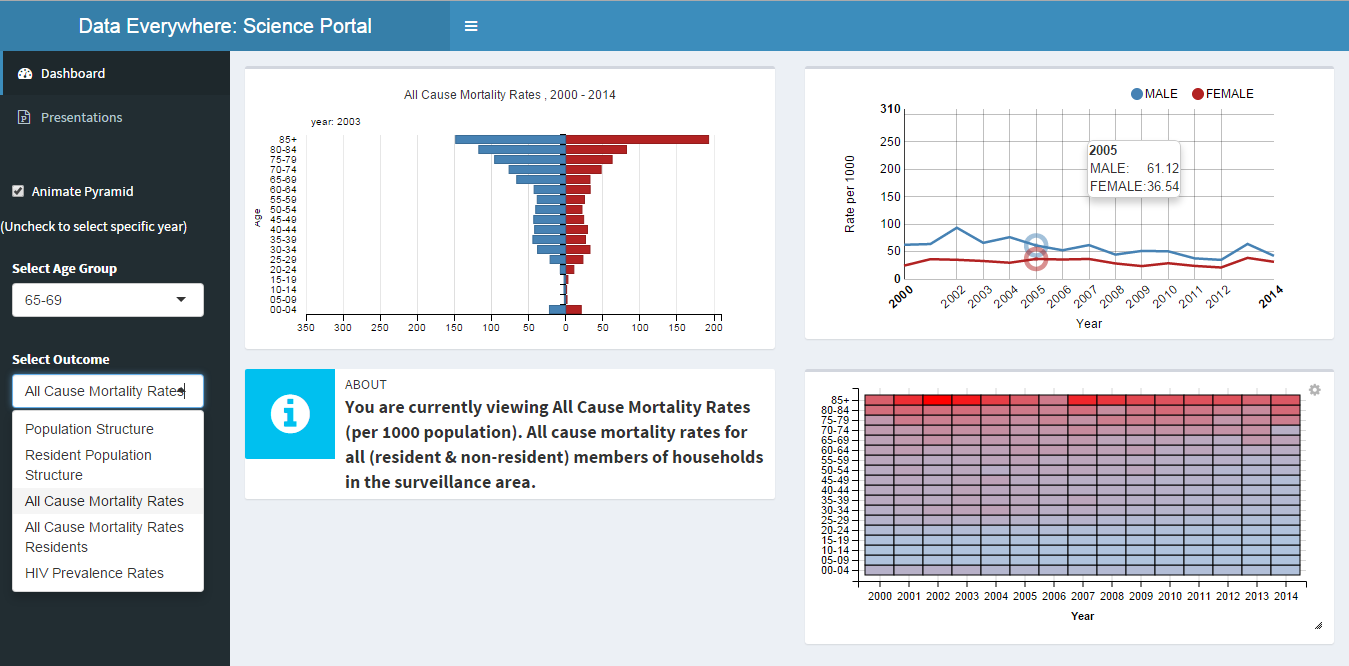
\includegraphics[scale=0.3]{./Chapter5/images/shinymp2}
\caption{MP graph showing All Cause Mortality Rate of a population in a particular health and demographic surveillance site}
\label{fig3}
\end{figure}

In \ref{fig3}, we see the same MP canvas showing a different outcome of interest, in this case All Cause Mortality Rate of the population at the Africa Centre Health and Demographic Surveillance System site. The outcome of interest is selected from a drop down menu on the left sidebar (in this graph it is visibly showing 5 possible outcomes to choose from, Population Structure, Resident Population Structure, All Cause Mortality Rates, All Cause Mortality Rates (Resident) and HIV Prevalence Rates). 

\section{Implementation of the Science Portal}

In this section we look at how we implement the Scientific Portal, from the data preparation, the programming algorithms used and the tools and technologies involved.

\subsection{Data Preparation}

The emphasis for the scientific portal was to create a solution which was generalizable enough to be moved to other INDEPTH sites and be integrated little to no modification to the software. The key to this was to make the scientific portal metadata driven, while following the data structures and conventions which we expand on here.  We use Pentaho Kettle transformations and jobs to perform all ETL tasks described here. 

The data is prepared in the three steps summarized below:

\begin{enumerate}
 \item Prepare an empty indicator lookup file
 \item Add an indicator $x$ entry into the indicator lookup file which includes in one of its fields the intended URI of the dataset for the indicator
 \item Generate the data for the indicator $x$ and place the data set at the URI indicated in step 2
\end{enumerate}

These steps are repeated for each new indicator which we would wish to visualise on the Scientific Portal. This is accomplished with a Pentaho Kettle transformation for each step, which is eventually incorporated into a Pentaho Kettle job for a single point of execution.

\subsubsection{Prepare indicator file}

The first step involves creating an empty indicator file as a Comma Separated Variable (csv) file. This is the lookup file for all indicators which we wish to visualize. The file follows a naming and structural convention which has to be followed as the application depends on these conventions. The file has the fields named $label, file, rate, multiplier$ and $description$. 

The $label$ field will hold the name of the indicator and will be used to populate the drop down menu on the user interface. The $file$ field will hold the URI location of the indicator and will be used to tell the application where to find the data related to a selected choice in the drop down menu. The $rate$ field will hold a Boolean value flagging whether the indicator is a rate or not. The $multiplier$ field is the constant value with which to multiply a calculated value if the indicator is flagged as a rate.The $description$ field will hold some descriptive text describing the indicator selected in the drop down menu.

\begin{figure}[!ht] 
\centering
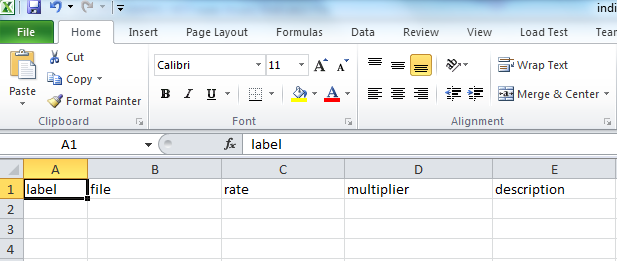
\includegraphics[scale=0.5]{./Chapter5/images/indicatorfile}
\caption{The initial empty indicator lookup file with the required fields}
\label{fig4}
\end{figure}